\section{Costruzione del Reticolo della Conoscenza}
\label{Costruzione del Reticolo della Conoscenza}
Dal 26/07 al 28/07 ho iniziato la Costruzione del Reticolo della Conoscenza. Per realizzarlo ho utilizzato un'applicativo sviluppato durante un precedente stage dell'azienda, che fa largo uso della libreria d3.js. Svolge elaborazione di dati, presentandoli in \textit{Cluster Based} o \textit{Force Based}, a discrezione delle esigenze dell'utente.\\
L'attivit\`a di creazione, documentazione e test del Reticolo \`e durata fino al termine dello stage.

\subsection{Descrizione del sistema}
\label{Descrizione del sistema}
L'applicazione accetta in import file di estensione CSV. Ogni colonna di quest'ultimo viene interpretata dal sistema come un parametro da elaborare; per questo la prima riga del file deve essere o preceduta da una dichiarazione di variabili, tante quante sono le colonne da parametrizzare, oppure \`e la prima riga di dati che viene interpretata come una dichiarazione e conseguentemente non rappresentata all'interno del Reticolo.\\
Nel sistema possono venire settati i seguenti aspetti:
\begin{itemize}
\item La \textit{tipologia} di Reticolo:
\begin{itemize}
\item Cluster Based: raggruppa un insieme di oggetti in modo tale che gli tutti gli elementi contenuti nel medesimo cluster sono pi\`u simili l'uno all'altro rispetto a quelli contenuti in altri gruppi;
\item Force Based: in base alla forza di ogni nodo, viene rappresentata come un'unica regione compatta le istanze appartenenti alla medesima classe, in cui vengono visivamente identificati i percorsi di differenziazione. Nel layout le celle differenzianti sono poste in prossimit\`a della classe pi\`u fortemente correlata.
\end{itemize}
\item \textit{Normalizzazione} dei dati in input:
\begin{itemize}
\item No: non viene applicata alcuna tecnica di normalizzazione dei dati;
\item MinMax: i dati vengono ridimensionati su un intervallo specifico (min, max), tuttavia tale tecnica non \`e in grado di gestire i valori anomali;
\item Gaussian: o normale in cui i dati vengono normalizzati in una curva, in cui i valori della stessa grandezza sono soggetti ad approssimazione;
\item Interquartile: si occupa di standardizzare i dati in modo da quantificare l'estensione del 50\% della distribuzione del carattere, che si trovano attorno alla mediana;
\end{itemize}
\item Tipologia di \textit{distanza} applicabili ai punti:
\begin{itemize}
\item Euclidea: tiene conto della distanza tra i punti;
\item Camberra: tiene conto della distanza tra le coppie in uno spazio vettoriale;
\item Pearson: distanza di correlazione che misura il grado di correlazione tra due punti. Valuta la covarianza tra due variabili in rapporto al prodotto della deviazione standard. Non \`e vantaggiosa su dati semplici.
\end{itemize}
\item \textit{Metodo} di associazione dei punti:
\begin{itemize}
\item Single: "vicino al prossimo", la distanza fra i gruppi \`e posta al pari della pi\`u piccola delle distanze calcolabili a due a due tra tutti gli elementi del gruppo. Accentua tutte le somiglianze tra i gruppi a discapito  della loro differenziazione netta.
\item Complete: "vicino pi\`u lontano", viene considerata la maggiore tra le distanze calcolate a due a due tra gli elementi di due gruppi. Privilegia la differenziazione tra i gruppi a discapito dell'omogeneit\`a degli elementi in essi contenuti. In questo caso i punti vengono rappresentati come meno compatti e diluiti.
\item Average: viene considerata come distanza fra due gruppi la media fra tutte le distanze calcolate a due a due tra gli elementi dei due gruppi. I risultati ottenibili sono i pi\`u attendibili (essendo basato sulla media delle distanze), i gruppi risultano pi\`u omogenei e differenziati tra di loro.
\end{itemize}
\end{itemize}
\noindent
Un'ulteriore funzionalit\`a, del applicativo, permette all'utente di decidere se si desidera procedere con una rappresentazione del Reticolo manuale o automatica progressiva.

\subsubsection{Configurazione}
\label{configurazione}
Analizzando l'applicativo in base al carattere dei miei dati in ingresso e alle aspettative sull'output del modello, ho valutato come configurazione pi\`u idonea per la formazione del Reticolo della Conoscenza \`e la seguente:
\begin{itemize}
\item \textit{Redistance}: No;
\item  \textit{Normalize}: No;
\item \textit{Distance-Type}: Euclidea;
\item \textit{Method}: Single.
\end{itemize}
\noindent
\begin{figure}[H]
\centering
	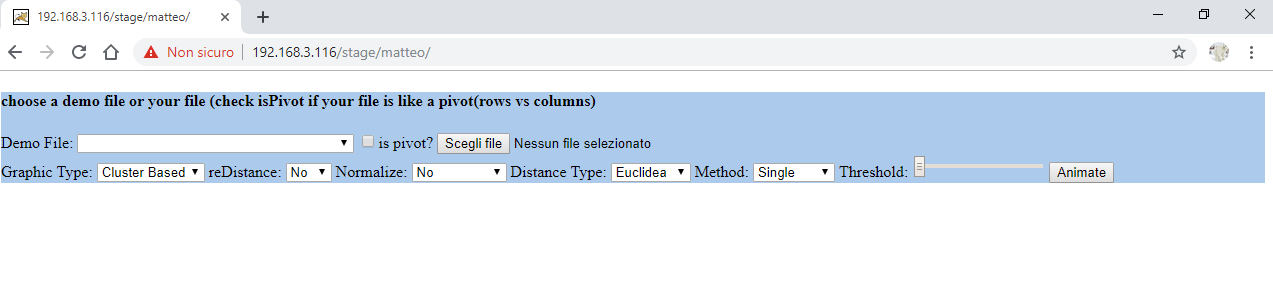
\includegraphics[width=1\linewidth]{./image/img-configurazione_reticolo.png}
	\caption{Configurazione usata nel sistema per generare il Reticolo della Conoscenza.}
	\label{Configurazione usata nel sistema per generare il Reticolo della Conoscenza.}
\end{figure}
\noindent

\subsection{Creazione dei file CSV}
\label{Creazione dei file CSV}
Come gi\`a accentato all'interno della sezione §{Descrizione del sistema} prima di procedere alla creazione del Reticolo, ho dovuto preparare i dati di previsione. Questo \`e stato reso pi\`u agevole grazie alla creazione, da parte mia, di un metodo che ha il compito, una volta messa in funzione la Rete neurale oggetto di studio (di prova o del database), di calcolare:
\begin{enumerate}
\item Le previsioni ottenibili da un vettore di previsione settato a 1 o -1 per ogni singolo elemento;
\item Sui dati del punto (1) un vettore delle differenze dove viene calcolato il delta in rapporto al vettore standard \footnote{Vettore tutto a zero}.
\end{enumerate}
\noindent
Ho fatto in modo che il vettore delle differenze venga stampato su console del browser \footnote{unica alternativa facendo uso di solo codice javascript}, in modo che ne basti prelevare il contenuto e inserirlo su un file CSV. Ogni elemento per poter funzionare all'interno dell'applicativo deve essere separato da un ; e ogni riga di previsione deve essere preceduta dal codice della domande in modo da rendere pi\`u agevole l'interpretazione del Reticolo. \`E a discrezione dell'utente l'inserimento di un'ulteriore riga di dichiarazione dei parametri.

\subsection{Creazione del Reticolo della Conoscenza per sui dati di Prova}
\label{Creazione del Reticolo della Conoscenza per sui dati di Prova}

\subsubsection{L'architettura della Rete}
\label{L'architettura della Rete}
Durante la costruzione del Reticolo della Conoscenza \`e stato importante capire se effettivamente l'architettura scelta in precedenza fosse corretta, e il suo vero significato. La rete sviluppata per il progetto \`e una Rete neurale statica a multistrato, nella quale sono presenti i seguenti elementi:
\begin{itemize}
\item input layer: dove viene dichiarata la dimensione dell'input: lunghezza, larghezza e profondit\`a dei dati da analizzare;
\item hidden layer (o layer intermedio): composto da uno o pi`u strati nascosti (o intermedi) costituito da m neuroni;
\item output layer:  costituito da p neuroni pari al numero di output desiderati.
\end{itemize}
\noindent 
Una Rete neurale permette di formulare complessi modelli matematici (sistemi di equazioni differenziali ecc.) e di individuarne possibili soluzioni. Le soluzioni si determinano sempre a partire dai dati; tuttavia la scelta del modello\footnote{inteso come architettura.} \`e un'azione molto complessa.

\noindent
\begin{figure}[H]
\centering
	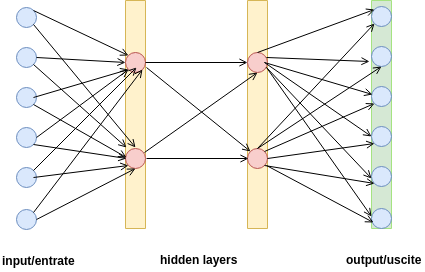
\includegraphics[width=0.60\linewidth]{./image/architettura-rete-prova.png}
	\caption{Archittettura delle Rete di prova: 6 ingressi in una rete a 3 strati con 2 stati nascosti e uscite.}
	\label{Archittettura delle Rete di prova: 6 ingressi in una rete a 3 strati con 2 stati nascosti e uscite.}
\end{figure}
\noindent


\noindent
\begin{figure}[H]
\centering
	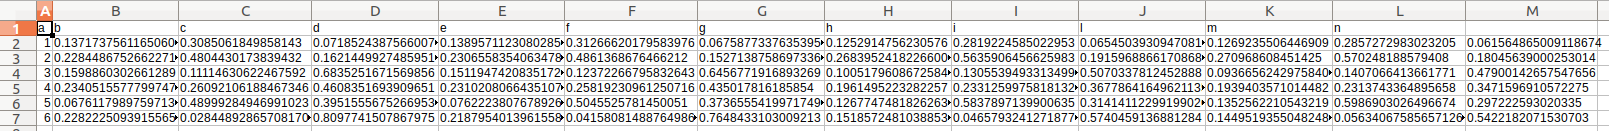
\includegraphics[width=1\linewidth]{./image/fileCSV_rete-prova.png}
	\caption{file CSV generato per la creazione del Reticolo della Conoscenza sui dati di prova.}
	\label{file CSV generato per la creazione del Reticolo della Conoscenza sui dati di prova.}
\end{figure}
\noindent

\subsubsection{Il Reticolo della Conoscenza generato}
\label{Il Reticolo della Conoscenza generato}

Di seguito sono riportate le sequenze di creazione del Reticolo della Conoscenza per i dati di prova.
\noindent

\begin{figure}[H]
\centering
	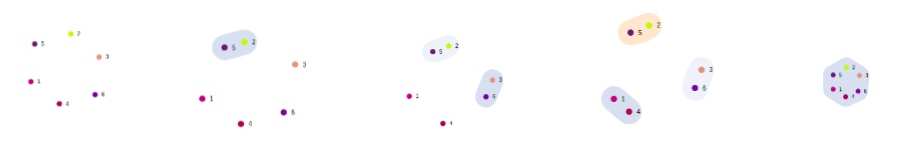
\includegraphics[width=1.20\linewidth]{./image/collage_reticolo-general-cluster.png}
	\caption{Reticolo della Conoscenza per i dati di prova - Cluster based.}
	\label{Reticolo della Conoscenza per i dati di prova - Cluster based.}
\end{figure}
\noindent

\begin{figure}[H]
\centering
	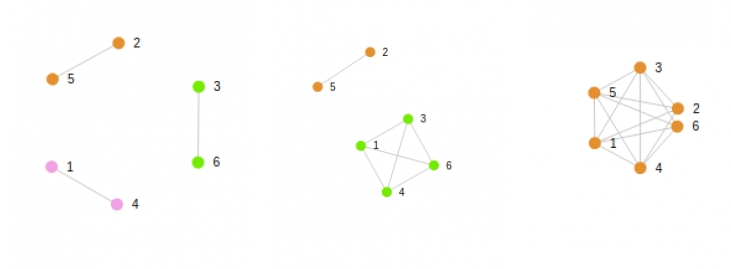
\includegraphics[width=1\linewidth]{./image/collage_reticolo-general-forced.png}
	\caption{Reticolo della Conoscenza per i dati di prova - Forced based.}
	\label{Reticolo della Conoscenza per i dati di prova - Forced based.}
\end{figure}
\noindent

\begin{figure}[H]
\centering
	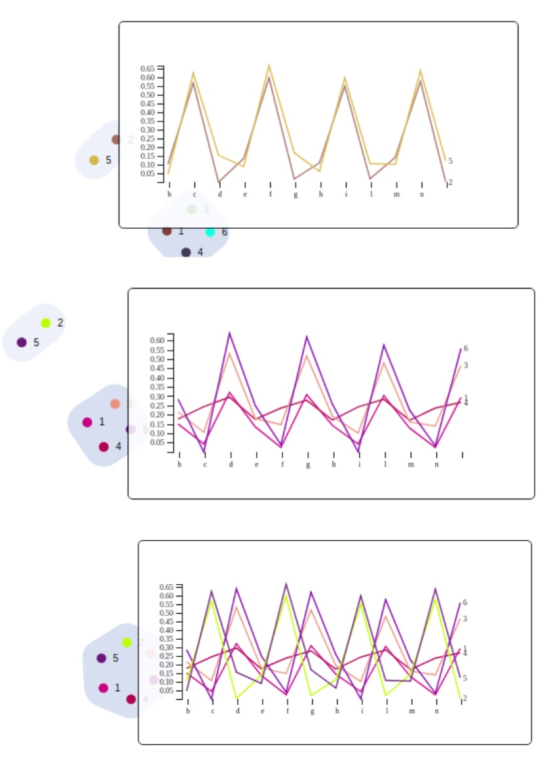
\includegraphics[width=0.50\linewidth]{./image/collage_reticolo-general-statistic.png}
	\caption{Reticolo della Conoscenza per i dati di prova - Statistiche.}
	\label{Reticolo della Conoscenza per i dati di prova - Statistiche.}
\end{figure}
\noindent
Appare come il Reticolo generato rispetta quando definito dalla figura \ref{Grafo rappresentante le relazioni esistenti tra il set di domande di prova.}.\\
Tuttavia effettuando delle ulteriori prove con file dati differenti; ma provenienti dalla medesima Rete neurale ho riscontrato situazioni contrastanti. L'errore osservato nei casi non corretti riguarda le coppie di domande 1, 4 e 3, 6. Un esempio del fenomeno \`e illustrato di seguito.\\\\
\noindent
La spiegazione del Reticolo malformato \`e da ricondurre alla natura stessa del vettori di input usati per l'addestramento della Rete di prova. Difatti i valori delle domande correlate sono i medesimi, solo se entrambe le domande sono state poste in fase di test, altrimenti quando la domanda \`e non posta viene valutata 0. Questo provoca un' oscillazione degli accoppiamenti genitori-figli. Tuttavia \`e solo un discostamento causato dalla frequenza con il quale le domande vengono poste di cui l'addestramento della Rete ne risente troppo e che  non riesce a mitigare del tutto; come si vede dalle figure seguenti.

\begin{figure}[H]
\centering
	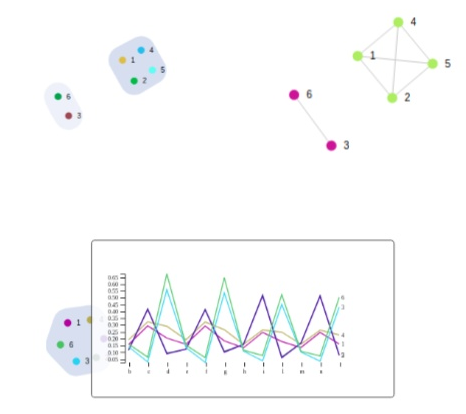
\includegraphics[width=0.60\linewidth]{./image/collage_reticolo-general-PROBLEMA.png}
	\caption{Reticolo della Conoscenza per i dati di prova - Presenza di valori di alterazione.}
	\label{Reticolo della Conoscenza per i dati di prova - Presenza di valori di alterazione.}
\end{figure}
\noindent
Le domande 6 e 3 sono state poste un numero superiore di volte rispetto alle domande figlie 1, 4, per cui il sistema associa le coppie 1, 4 con le coppie 2, 5 che hanno tra loro una frequenza, dei valori iniziali, pi\`u vicina. Inoltre vi \`e da dire che il metodo Sinple usato dall'applicativo per associare le domande, nel momento in cui correla tra loro due punti, il prossimo punto viene calcolato dal complessivo, invece che dal punto con una distanza appena superiore al punto appena Single. Quest'ultimo punto avr\`a un impatto superiore tanto pi\`u sono grandi le dimensioni del Reticolo.
Per valutare al meglio l'impatto che di quanto affermato sopra, in fase di test mi sono preoccupata di analizzare e come si comporta la Rete neurale, relativa ai dati di prova, considerando esclusivamente la possibilit\`a che un candidato o risponda correttamente ad una domanda (1) o la sbagli (-1). I risultati di previsione ottenuti sono i seguenti:
\begin{figure}[H]
\centering
	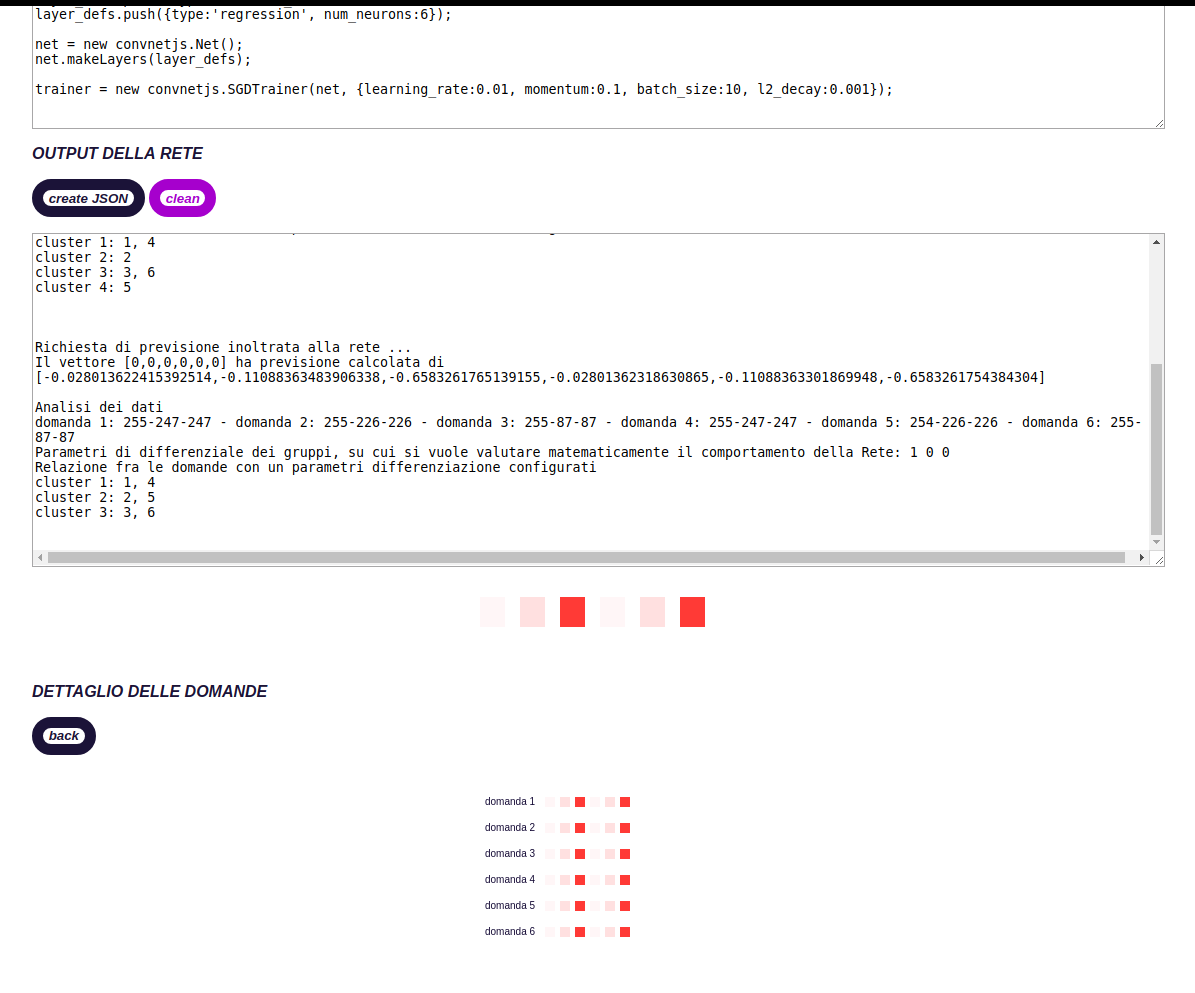
\includegraphics[width=1\linewidth]{./image/RetediProva_generatorinputpuro.png}
	\caption{Risultati della Rete di prova con un set di dati puro (esclusivamente 1 e -1).}
	\label{Risultati della Rete di prova con un set di dati puro (esclusivamente 1 e -1).}
	\end{figure}
	\noindent
Come si pu\`o vedere dalla figura \ref{Risultati della Rete di test con un set di dati puro (esclusivamente 1 e -1).} le previsioni ottenute per le coppie di domande (1;4), (3;6) e (2;5) sono identiche, ad eccezioni di alcune variazioni impercettibili da ricondurre ad oscillazioni di Rete e che non hanno alcun impatto sui risultati da raggiungere. Impostando di ottenere una previsione sul valore 0 e avendo allenato la Rete esclusivamente con valori -1 e 1 mi aspetto che venga effettuata la media, ed \`e quello che viene fatto effettivamente, per tutte le domande coinvolte. dalla Rete.
Il fenomeno sorprendente, che mette in luce l'importanza di avere un valore 0 di risposta (non data) nel trainset, \`e mostrato nelle figure sotto.
\begin{figure}[H]
\centering
	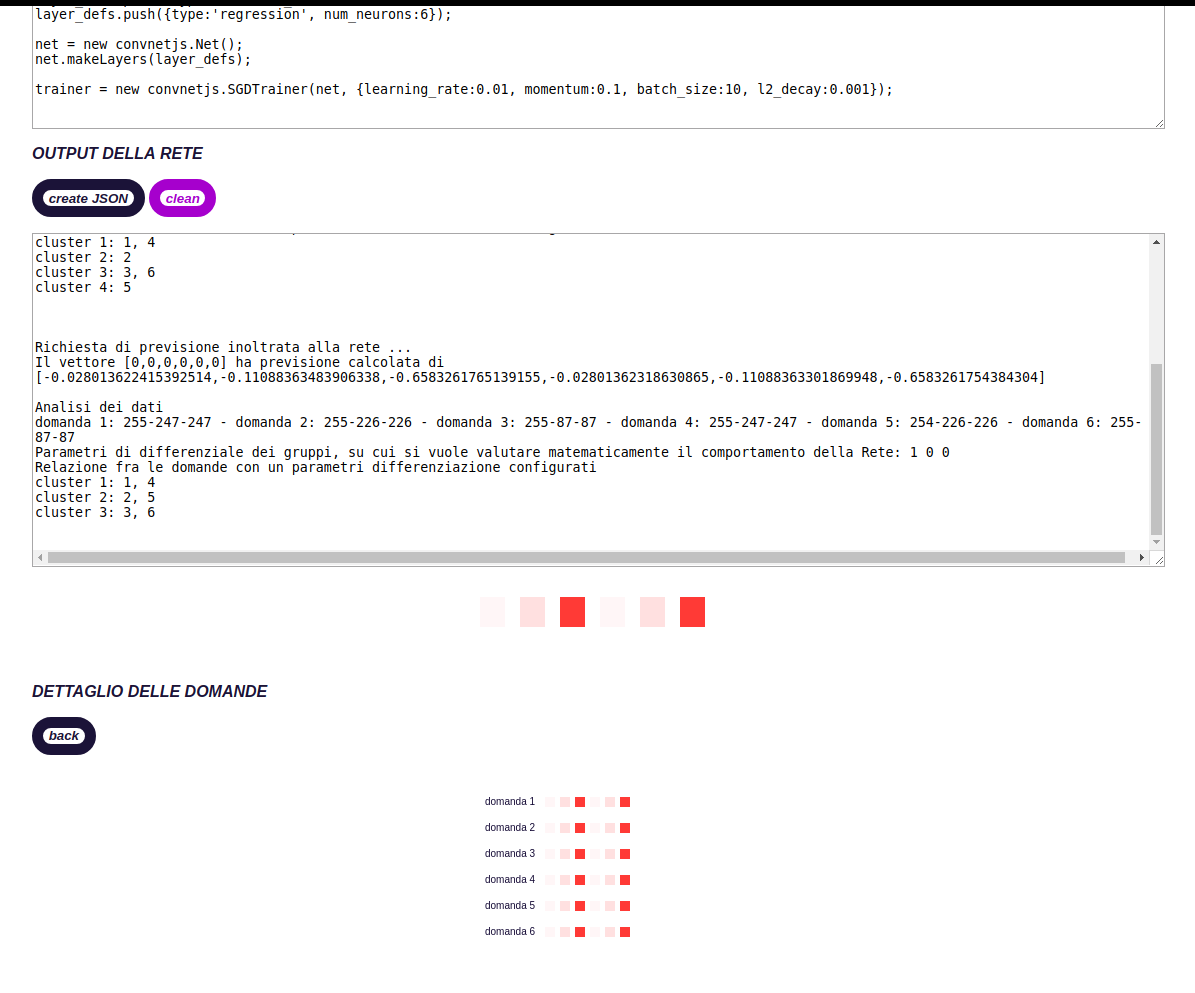
\includegraphics[width=1\linewidth]{./image/RetediProva_generatorinputpuro.png}
	\caption{Risultati della Rete di test con un set di dati puro (esclusivamente 1 e -1), vettore previsione [-1, 0, 0, 0, 0, 0].}
	\label{Risultati della Rete di test con un set di dati puro (esclusivamente 1 e -1), vettore previsione [-1, 0, 0, 0, 0, 0].}
\end{figure}
\noindent

\begin{figure}[H]
\centering
	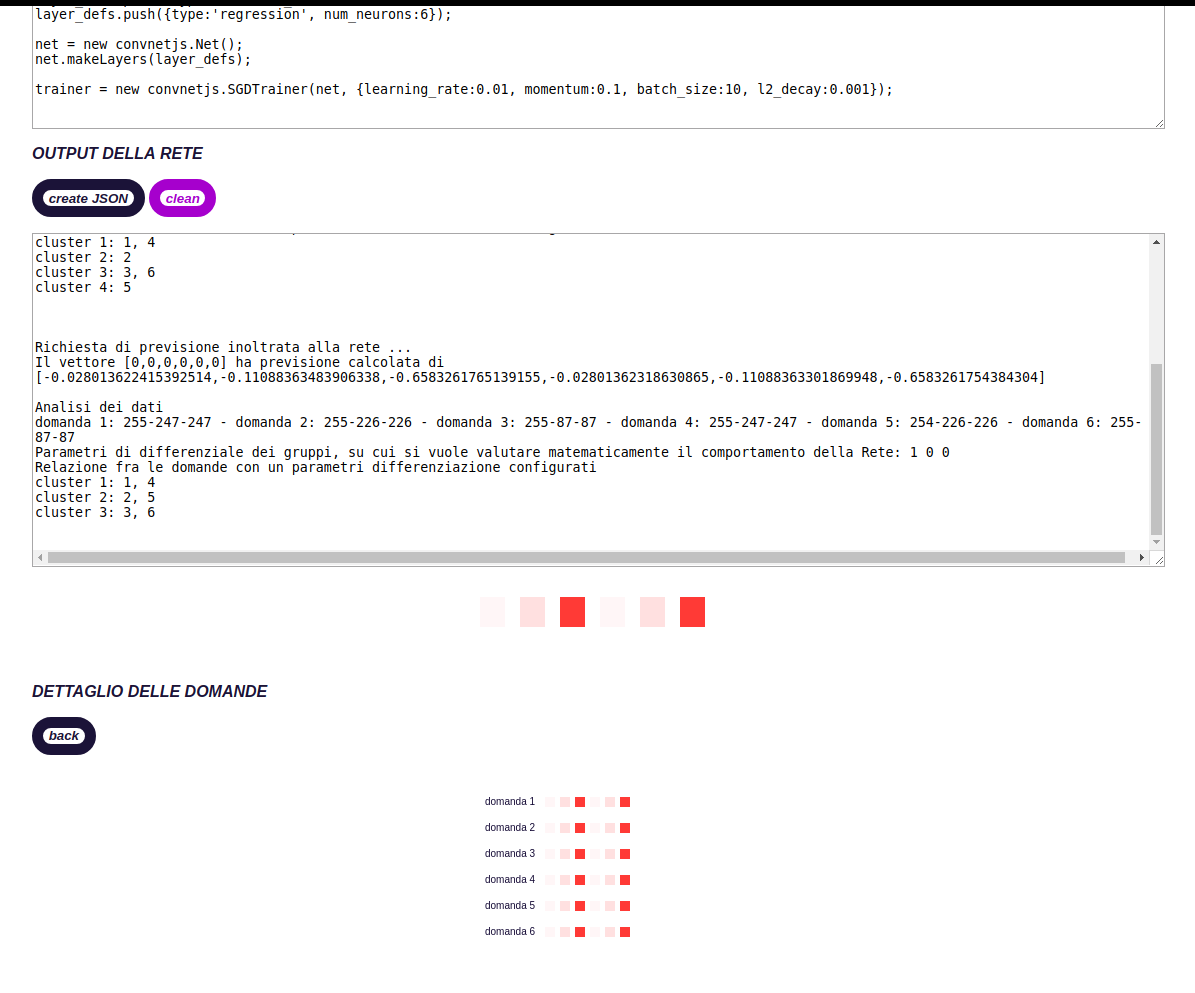
\includegraphics[width=1\linewidth]{./image/RetediProva_generatorinputpuro.png}
	\caption{Risultati della Rete di test con un set di dati puro (esclusivamente 1 e -1), vettore previsione [0, 0, 0, -1, 0, 0].}
	\label{Risultati della Rete di test con un set di dati puro (esclusivamente 1 e -1), vettore previsione [0, 0, 0, -1, 0, 0].}
\end{figure}
\noindent
Non avere un valore a 0 porta le le previsioni imposte alle singole domande, valutate in coppia, a mostrare come unica relazione stretta esistente la coppia coinvolta, scollegando ogni relazione con le altre coppie. Ad esempio, le domande 2 e 4 vengono colorate di verdino nella previsione della domanda 1 e di rosso nella domanda 4. Questo ha un'inpatto sulla previsione visiva della Rete, dal quale risulta impossibile la previsione di domande figlie e genitori.\\
La matrice correlazione ottenuta, tuttavia dal modello della PCA, risulta perfettamente allineata con le aspettative delle coppie di domande e delle previsioni, tuttavia questo \`e possibile solo perch\`e i dati e le previsioni vengono valutati nella loro generalit\`a e non tra coppia di domande.


\subsubsection{Valutazione con la frequenza}
\label{Valutazione con la frequenza}
Ho ritenuto adeguato studiare il comportamento dei set di dati anche in base alla loro frequenza; in modo da poterne valutare le differenze con la Rete neurale e se vi fossero benefici o meno.\\
Come primo passo ho provveduto a calcolarmi per ogni domanda quale fosse la frequenza delle altre domande valutate in accordo e in disaccordo con la risposta data. Ho effettuato il procedimento sia nel caso di una domanda risposta correttamente che non.\\\\
\noindent
Il Reticolo generato rispetta fedelmente le aspettative, definite dal Grafo della Conoscenza in figura ref{Grafo rappresentante le relazioni esistenti tra il set di domande di prova}. Tuttavia questo non va valutato come un risultato positivo, in quanto indicatore che ai valori -1, che dovrebbero alterare, anche se marginalmente, il risultato finale non viene data l'adeguata importanza. Il beneficio dell'uso della Rete sta proprio in quest'ultimo fattore, con l'impiego dell'apprendimento vengono rilevate situazioni che la sola frequenza non \`e in grado di pesare.

\begin{figure}[H]
\centering
	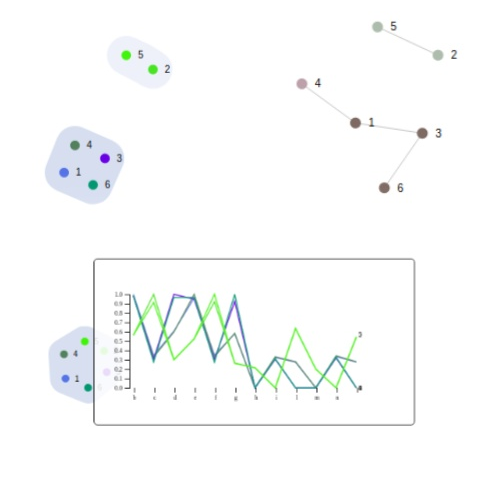
\includegraphics[width=0.50\linewidth]{./image/collage_reticolo-general-FREQ.png}
	\caption{Reticolo della Conoscenza per i dati di prova - Frequenza.}
	\label{Reticolo della Conoscenza per i dati di prova - Frequenza.}
\end{figure}
\noindent


\subsubsection{Osservazioni}
\label{Osservazioni Reticolo dati di prova}
In conclusione il Reticolo della Conoscenza, costruito per mezzo delle previsioni della Reten neurale, anche se non sempre perfettamente coerente con le aspettative; nella maggioranza dei casi ricalca fedelmente quanto evidenziato nella figura \ref{Grafo rappresentante le relazioni esistenti tra il set di domande di prova.} nella sezione § \ref{Test effettuati}. \\
Quando il Reticolo non \`e soggetto a deviazioni, gli accoppiamenti tra i punti, ricalcano fedelmente quanto dichiarato dalla matrice correlazione ottenuta dal modello generato dall'uso della PCA, e visibile dall'immagine \ref{CSV generato a partire dalla matrice correlazione del set della rete di prova.}.
\`E obbligo precisare, tuttavia che i risultati della PCA non devono essere presi come assioma assoluto. Le argomentazioni sono le seguenti:
\begin{itemize} 
\item La Rete neurale, pu\`o cogliere oscillazioni che il modello matematico non \`e in grado, e questo va ad invalidare i risultati ottenuti non solo dalla matrice correlazione, ma anche dell'individuazione dei punti sulle prime due componenti;
\item La PCA, come si \`e visto accadere con la frequenza, non tiene conto del numero di volte cui si verifica un evento attribuendone il medesimo peso. Invece la Rete, neurale mediante apprendimento, riesce a valutare al meglio tali fenomeni avvicinandosi il pi\`u possibile alla realt\`a.
\item Lo scopo principale della PCA \`e quello di spostare gli assi di rappresentazione degli eventi. in modo che vi sia una maggiore facilit\`a di comprensione dei dati, come si ha con standardizzazione dei valori.
\end{itemize}

\subsection{Creazione del Reticolo della Conoscenza sui dati delle domande nel database}
\label{Creazione del Reticolo della Conoscenza sui dati delle domande nel database}

La creazione del Reticolo della Conoscenza sui dati delle domande nel database ha richiesto la creazione di file CSV su un architettura a 2 layer della rete con 6, 8, 10, 12 neuroni ciascuno. Questo a causa della non conoscenza a priori del numero di cluster che comporranno il Reticolo, come invece accade per i dati di prova.\\
Tale differenziazione ha permesso durante la configurazione del sistema e la creazione del Reticolo che mi accorgersi dell'estrema variabilit\`a dei cluster e correlazioni a seconda dell'oscillazione del numero di neuroni per layers, come viene evidenziato dalle immagini seguenti.


\subsection{Osservazioni}
\subsubsection{Osservazioni Reticolo dati del database}
La variazione dei Reticoli ottenuti dalle diverse architetture della Rete neurale indica come sia necessario approfondire la tematica e individuare una strategia unica che permetta di individuare in modo univoco l'architettura necessaria per ottenere un Reticolo della Conoscenza valido.

\subsection{Creazione del Reticolo prendendo in considerazione le frequenze alle domande}
\label{Creazione del Reticolo prendendo in considerazione le frequenze alle domande}



\noindent
\begin{figure}[H]
\centering
	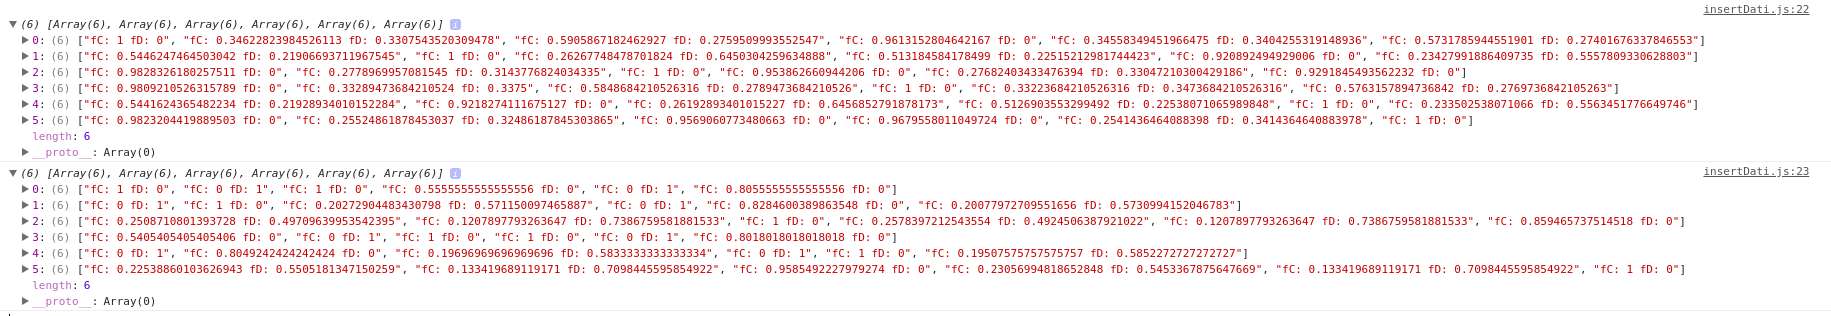
\includegraphics[width=1\linewidth]{./image/res_frequenceMatrix_OSS.png}
	\caption{Frequenza delle domande dei dati di test.}
	\label{Frequenza delle domande dei dati di test.}
\end{figure}
L'immagine sopra mostra per ogni domanda valutata a 1 (primo set di dati) e a -1 (secondo set di dati) la frequenza che intercorre in tutte le domande con segno coerente o opposto a quello della domanda in esame.
Il set di dati viene generato randomicamente con guida \footnote{con impiego del Grafo della Conoscenza (mostrato in figura \ref{Grafo rappresentante le relazioni esistenti tra il set di domande di prova.})}.
Analizzando i risultati di frequenza osservati ho riscontrato i seguenti fenomeni:
\begin{itemize}
\item Considerando i valori per riga:
\begin{itemize}
\item per le domande in cui le risposte si presentano corrette i valori di frequenza correlata e opposta si presentano con la seguente struttura:
\begin{itemize}
\item la domanda 3  si presenta con una frequenza correlata che coinvolge le coppie (1,3) e (4,6);
\item la domanda 6 si presenta con una frequenza correlata che coinvolge le coppie (1,6) e (4,3).
\end{itemize}
\item per le domande in cui le risposte si presentano sbagliate i valori di frequenza correlata e opposta si presentano con la seguente struttura:
\begin{itemize}
\item la domanda 1 si presenta con una frequenza correlata che coinvolge le coppie (1 ~ FC:1, 3 ~ FC:1) e (4 ~ FC:0.55, 6 ~ FC:0.80);
\item la domanda 4 si presenta con una frequenza correlata che coinvolge le coppie (4 ~ FC:1, 3 ~ FC:1) e (1 ~ FC:0.54, 6 ~ FC:0.80);
\end{itemize}
\end{itemize}
\item Considerando i valori per colonna:
\begin{itemize}
\item la domanda 1 si correla con la domanda 4;
\item la domanda 3 si correla con la domanda 6, 
\item la domanda 2 con la domanda 5.
\end{itemize}
\end{itemize}
\noindent
Tali considerazioni non sono esclusive per il singolo set di dati; ma rimangono costanti per ogni set di dati generato (anche se di natura parzialmente randomica). Ho riscontrato per ciascuna variabile al massimo un oscillazione che si attesta mai superiore a 0.2. Percui tali risultati risultano stabili e attendibili.
\\\\
I valori di frequenza possono concorrere alla formazione del Reticolo della Conoscenza. Per renderlo possibile ho provveduto ha creare un file csv che contenesse per ognuna delle domande tutte le domande coinvolte valutate con frequenze positive correlate e opposte e le frequenze negative correlate e opposte. La tecnica permette la generazione, per ogni domanda, di un vettore contenete un quantit\`a di dati 4 volte la dimensione dell'input/output della Rete.
Il divario permette, positivamente, di poter costruire un Reticolo ove i dati per ogni nodo hanno una stabilit\`a concreta.\\
Tuttavia il Reticolo generato riscontra delle peculiarit\`a:
\begin{itemize}
\item la frequenza non effettua alcuna riduzione dimensionale provocando uno utilizzo di spazio pari al numero di domande/dati da analizzare. Ci\`o comporta che per grandi moli da dati lo spazio necessario cresce elevato al numero di elementi di input;
\item la frequenza funziona male sui valori anomali, come gi\`a spiegato nella sezione § \ref{Descrizione del sistema}
\end{itemize}
\noindent
Il divario tra i valori per riga e colonna sono legittimati dalla natura del set di valori di input. In esso sono contenuti valori 0, e non esclusivamente -1 e 1, causa diretta dell'oscillazione delle correlazioni strette esistente tra le domande accoppiate \footnote{per i dati di prova le domande accoppiate sono (1;4), (3;6) e (2;5)}. La prova di quanto appena detto \`e evidente testando pi\`u volte la Rete. Per un n molto piccolo le previsioni, ottenute, risultano cos\`i vicine l'una all'altra che almeno 4 domande formano un unico cluster.
Tale curvatura dei dati ha il suo impatto peggiore sulle domande figlie e genitori. Le domande estranee vengono associate prima hai figli esclusivamente perch\`e molto semplici. Tuttavia l'oscillazione in esame \`e minima e il Reticolo ne risente esclusivamente quando i valori di previsione delle domande sono simili, motivo per cui in figura le colonne e le righe 2 e 5 risultano sempre conformi. 





